\documentclass[11pt,a4paper]{article}
\usepackage[utf8]{inputenc}
\usepackage{amsmath,amsfonts,amssymb}
\usepackage{graphicx}
\usepackage{geometry}
\geometry{margin=1in}
\usepackage{booktabs}
\usepackage{hyperref}
\usepackage{float}
\usepackage{xcolor}

\title{\textbf{EE3621: Digital Signal Processing} \\ \Large Lecture 5: Z-Transform, ROC \& Common Pairs \\ \large (III B.Tech EEE)}
\author{Lecture Notes (40-Minute Plan)}
\date{}

\definecolor{darkbg}{HTML}{0d121f}
\definecolor{lighttext}{HTML}{e2e8f0}
\definecolor{primary}{HTML}{8b5cf6}
\definecolor{secondary}{HTML}{0dd5c5}

\pagecolor{darkbg}
\color{lighttext}

\hypersetup{
    colorlinks=true,
    linkcolor=secondary,
    urlcolor=secondary
}

\begin{document}

\maketitle

\section{Lecture Plan \& Objectives (40 Minutes Breakdown)}
\begin{itemize}
    \item \textbf{00:00 -- 08:00 (8 mins):} Motivation: Z-transform as a generalization of the DTFT ($z = r e^{j\omega}$) and convergence proof.
    \item \textbf{08:00 -- 16:00 (8 mins):} The Region of Convergence (ROC): Does ROC lie inside the unit circle? Causal vs. Anti-causal vs. Two-sided shapes and Stability Comments.
    \item \textbf{16:00 -- 26:00 (10 mins):} Worked Examples: Exp, Sin, Cos, Unit Step, Impulse, and Multi-Pole Multi-Zero System (Magnitude \& Phase Computation).
    \item \textbf{26:00 -- 34:00 (8 mins):} Properties of the Z-Transform with full algebraic proofs.
    \item \textbf{34:00 -- 38:00 (4 mins):} Comprehensive Common Z-Transform Pairs Table.
    \item \textbf{38:00 -- 40:00 (2 mins):} Checkpoint and Concept Recap.
\end{itemize}

\noindent\rule{\textwidth}{0.5pt}

\section{Definition \& Mathematical Motivation}
The Z-transform of a discrete-time sequence $x[n]$ is defined as:
\begin{equation}
X(z) = \sum_{n=-\infty}^{\infty} x[n] z^{-n}
\end{equation}
Expressing $z$ in polar form $z = r e^{j\omega}$:
\begin{equation}
X(r e^{j\omega}) = \sum_{n=-\infty}^{\infty} (x[n] r^{-n}) e^{-j\omega n}
\end{equation}
Evaluating $X(z)$ on the unit circle ($|z|=1 \implies r=1$) yields the Discrete-Time Fourier Transform (DTFT): $X(z)\Big|_{|z|=1} = X(e^{j\omega})$.
The Z-transform series converges absolutely if:
\begin{equation}
\sum_{n=-\infty}^{\infty} |x[n] r^{-n}| < \infty
\end{equation}
The set of complex values $z$ for which this summation converges defines the \textbf{Region of Convergence (ROC)}.

\section{Properties of the ROC \& Unit Circle Location Clarification}

\subsection{Does the ROC Lie Inside the Unit Circle?}
Whether an ROC lies inside the unit circle depends directly on signal causality and pole magnitude:
\begin{enumerate}
    \item \textbf{Anti-Causal (Left-Sided) Signals:} The ROC is an \textbf{interior disk} $|z| < |p|_{min}$. If $|p| < 1$ (e.g., $p = 0.7$), the ROC is $|z| < 0.7$, which \textbf{lies entirely INSIDE the unit circle ($|z| < 1$)}.
    \item \textbf{Causal (Right-Sided) Signals:} The ROC is an \textbf{exterior domain} $|z| > |p|_{max}$ extending to infinity.
    \item \textbf{Two-Sided Signals:} The ROC is an \textbf{annular ring} $r_1 < |z| < r_2$.
    \item \textbf{BIBO Stability Criterion:} An LTI system is BIBO stable if and only if the ROC \textbf{contains the unit circle} ($|z|=1$).
\end{enumerate}

\begin{figure}[H]
\centering
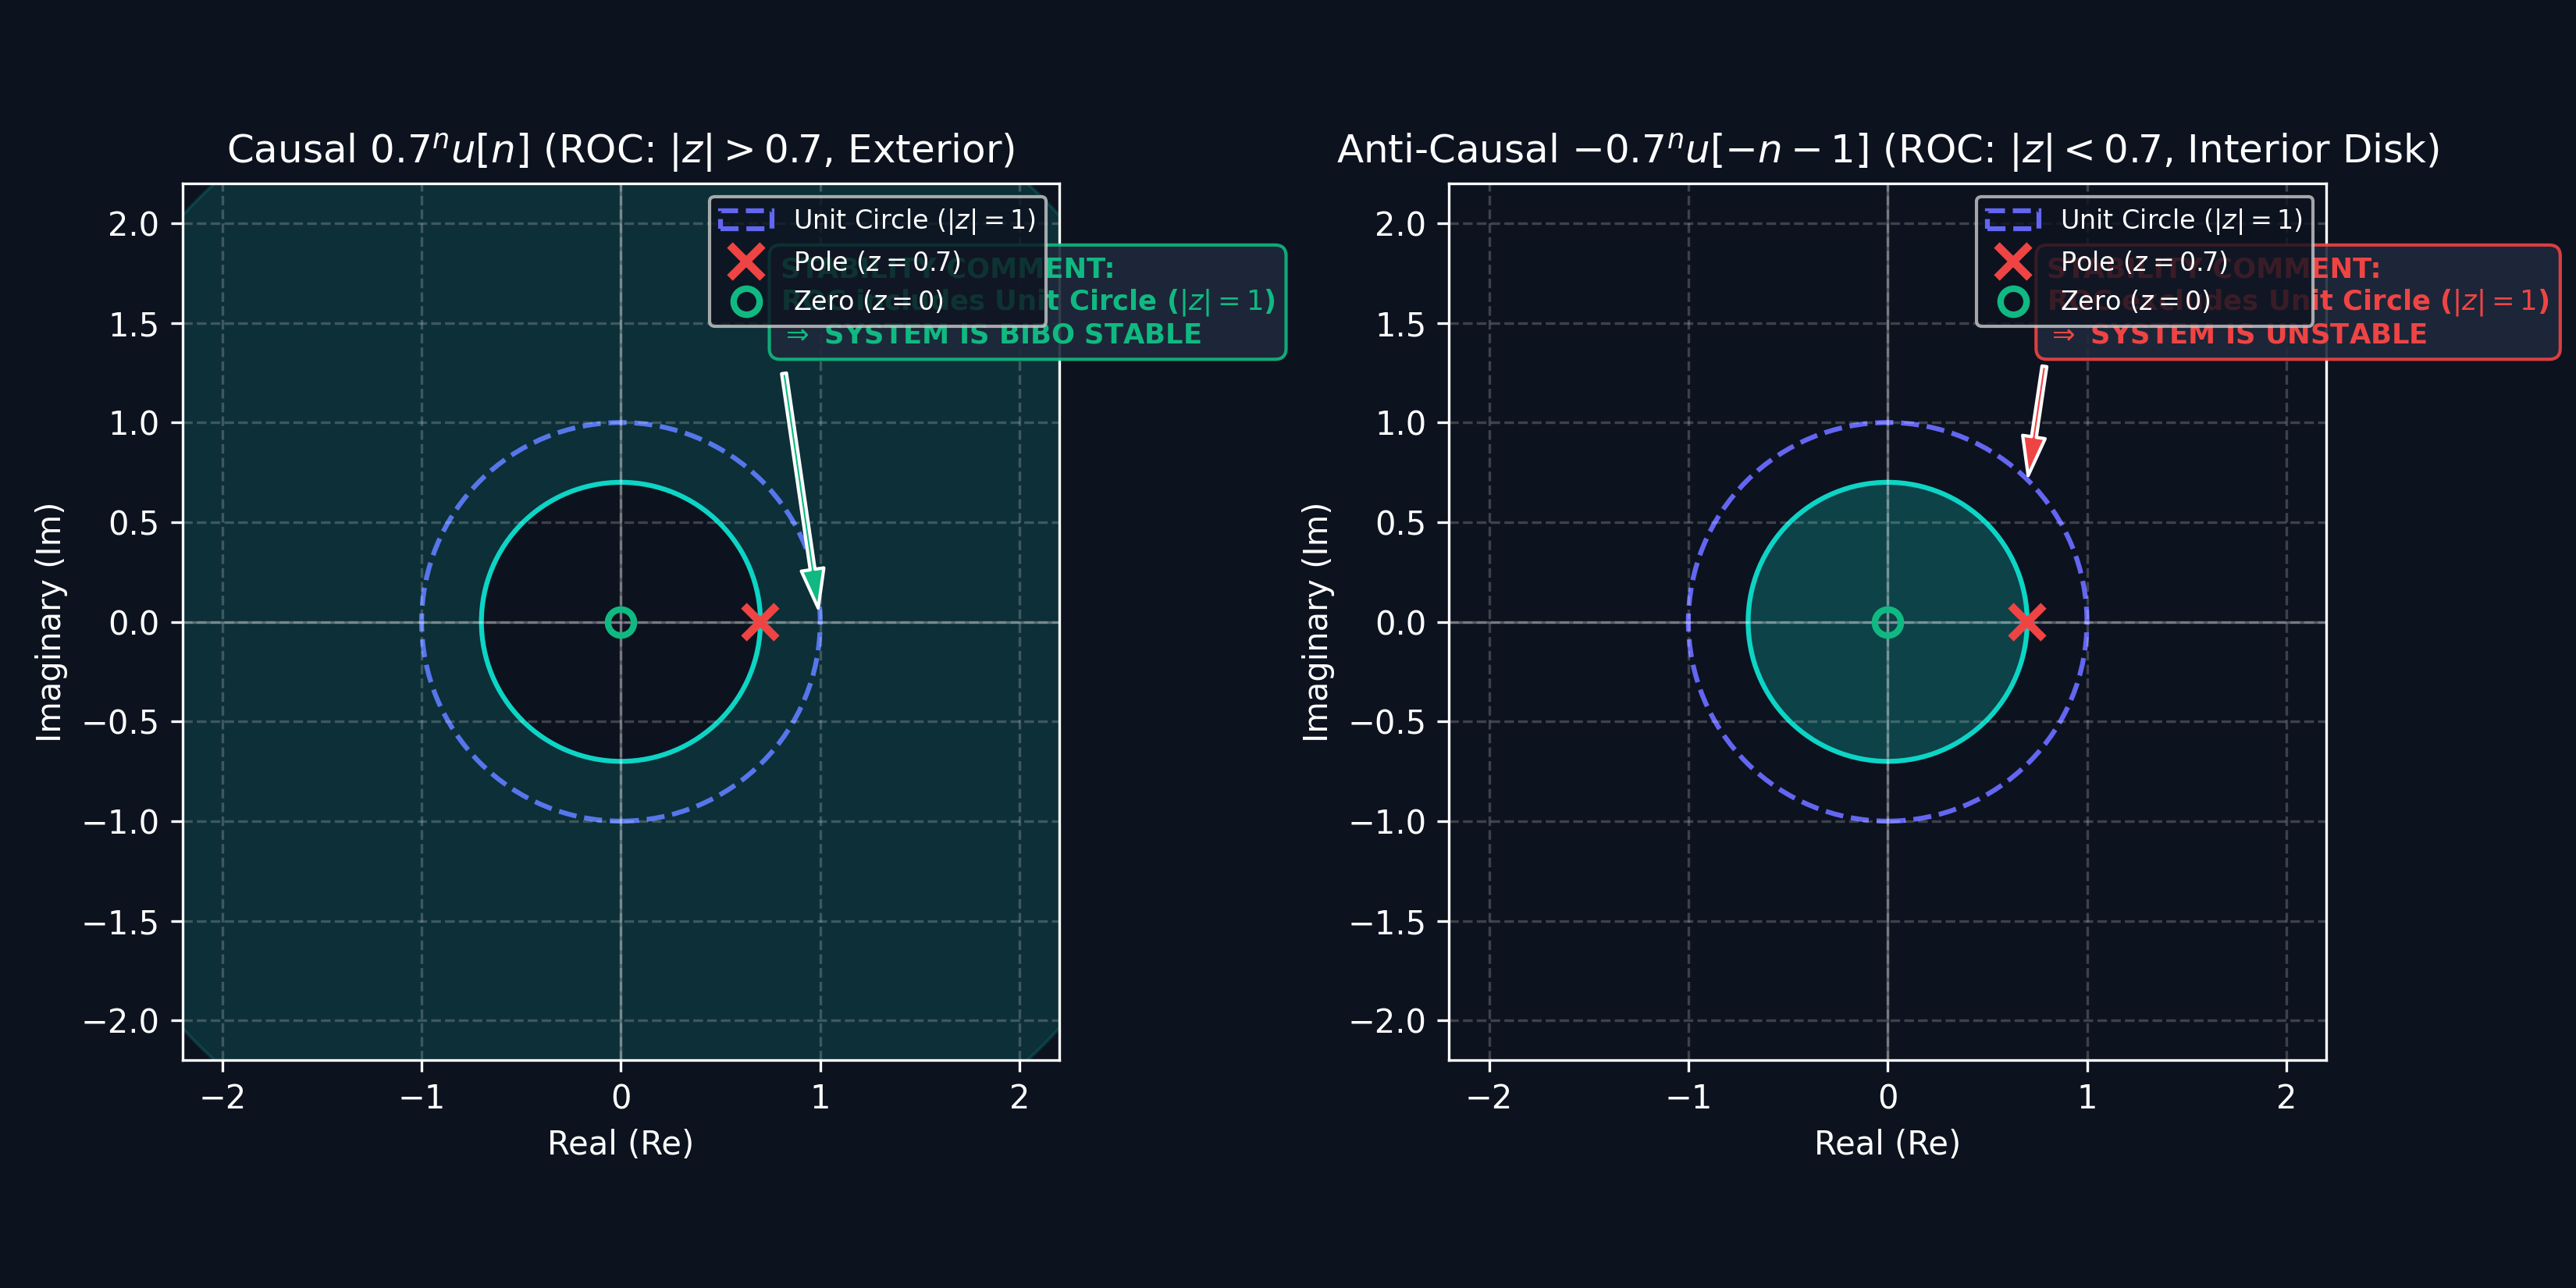
\includegraphics[width=0.85\textwidth]{images/roc_causal_anticausal.png}
\caption{ROC geometries in the z-plane for causal ($|z| > 0.7$) vs. anti-causal ($|z| < 0.7$, inside unit circle) signals with explicit BIBO stability comments.}
\label{fig:roc_causal}
\end{figure}

\section{Worked Examples: Signal Variants \& Multi-Pole Multi-Zero Systems}

\begin{figure}[H]
\centering
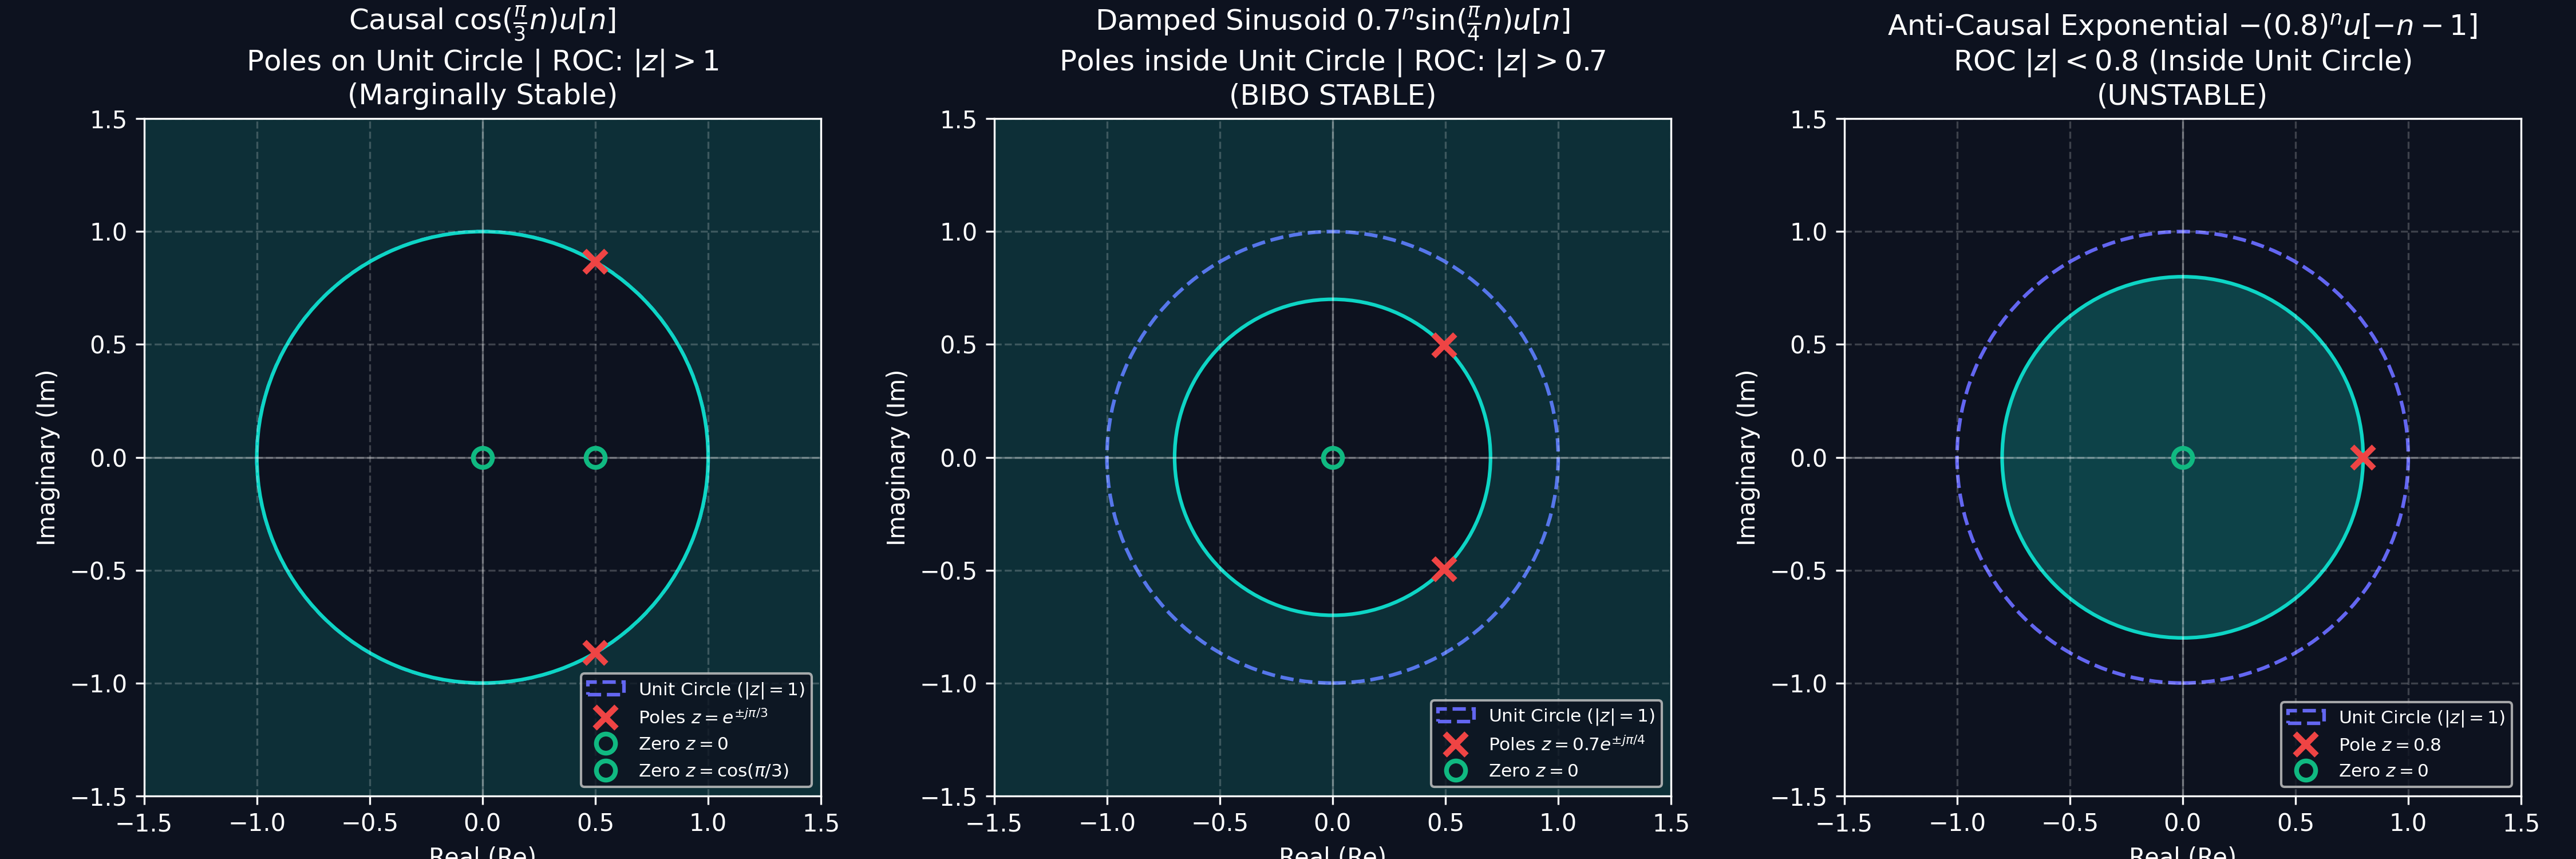
\includegraphics[width=0.95\textwidth]{images/pole_zero_roc_examples.png}
\caption{Demonstrative Pole-Zero plots and ROC regions for Causal Cosine, Damped Sinusoid, and Anti-Causal Exponential.}
\label{fig:pole_zero_examples}
\end{figure}

\subsection{Example 1: Impulse, Step, Cosine \& Damped Sinusoid}
\begin{itemize}
    \item \textbf{Unit Impulse $\delta[n]$:} $X(z) = 1$, ROC: All $z$. \textbf{Stable}.
    \item \textbf{Unit Step $u[n]$:} $X(z) = \frac{z}{z-1}$, Pole at $z=1$, ROC: $|z|>1$. \textbf{Marginally Stable}.
    \item \textbf{Cosine $\cos(\omega_0 n) u[n]$:} $X(z) = \frac{z(z - \cos\omega_0)}{z^2 - 2\cos\omega_0 z + 1}$, Poles at $z = e^{\pm j\omega_0}$ (on unit circle), ROC: $|z|>1$. \textbf{Marginally Stable}.
    \item \textbf{Damped Sinusoid $r_0^n \sin(\omega_0 n) u[n]$ ($r_0=0.7, \omega_0=\pi/4$):} $X(z) = \frac{0.7 \sin(\pi/4) z}{z^2 - 1.4 \cos(\pi/4) z + 0.49}$, Poles at $z = 0.7 e^{\pm j\pi/4}$, ROC: $|z|>0.7$. \textbf{BIBO Stable}.
\end{itemize}

\subsection{Example 2: Multi-Pole Multi-Zero System (ROC, Magnitude \& Phase)}
Consider $H(z) = \frac{z - 0.5}{z^2 - 0.8 z + 0.25}$.

\begin{figure}[H]
\centering
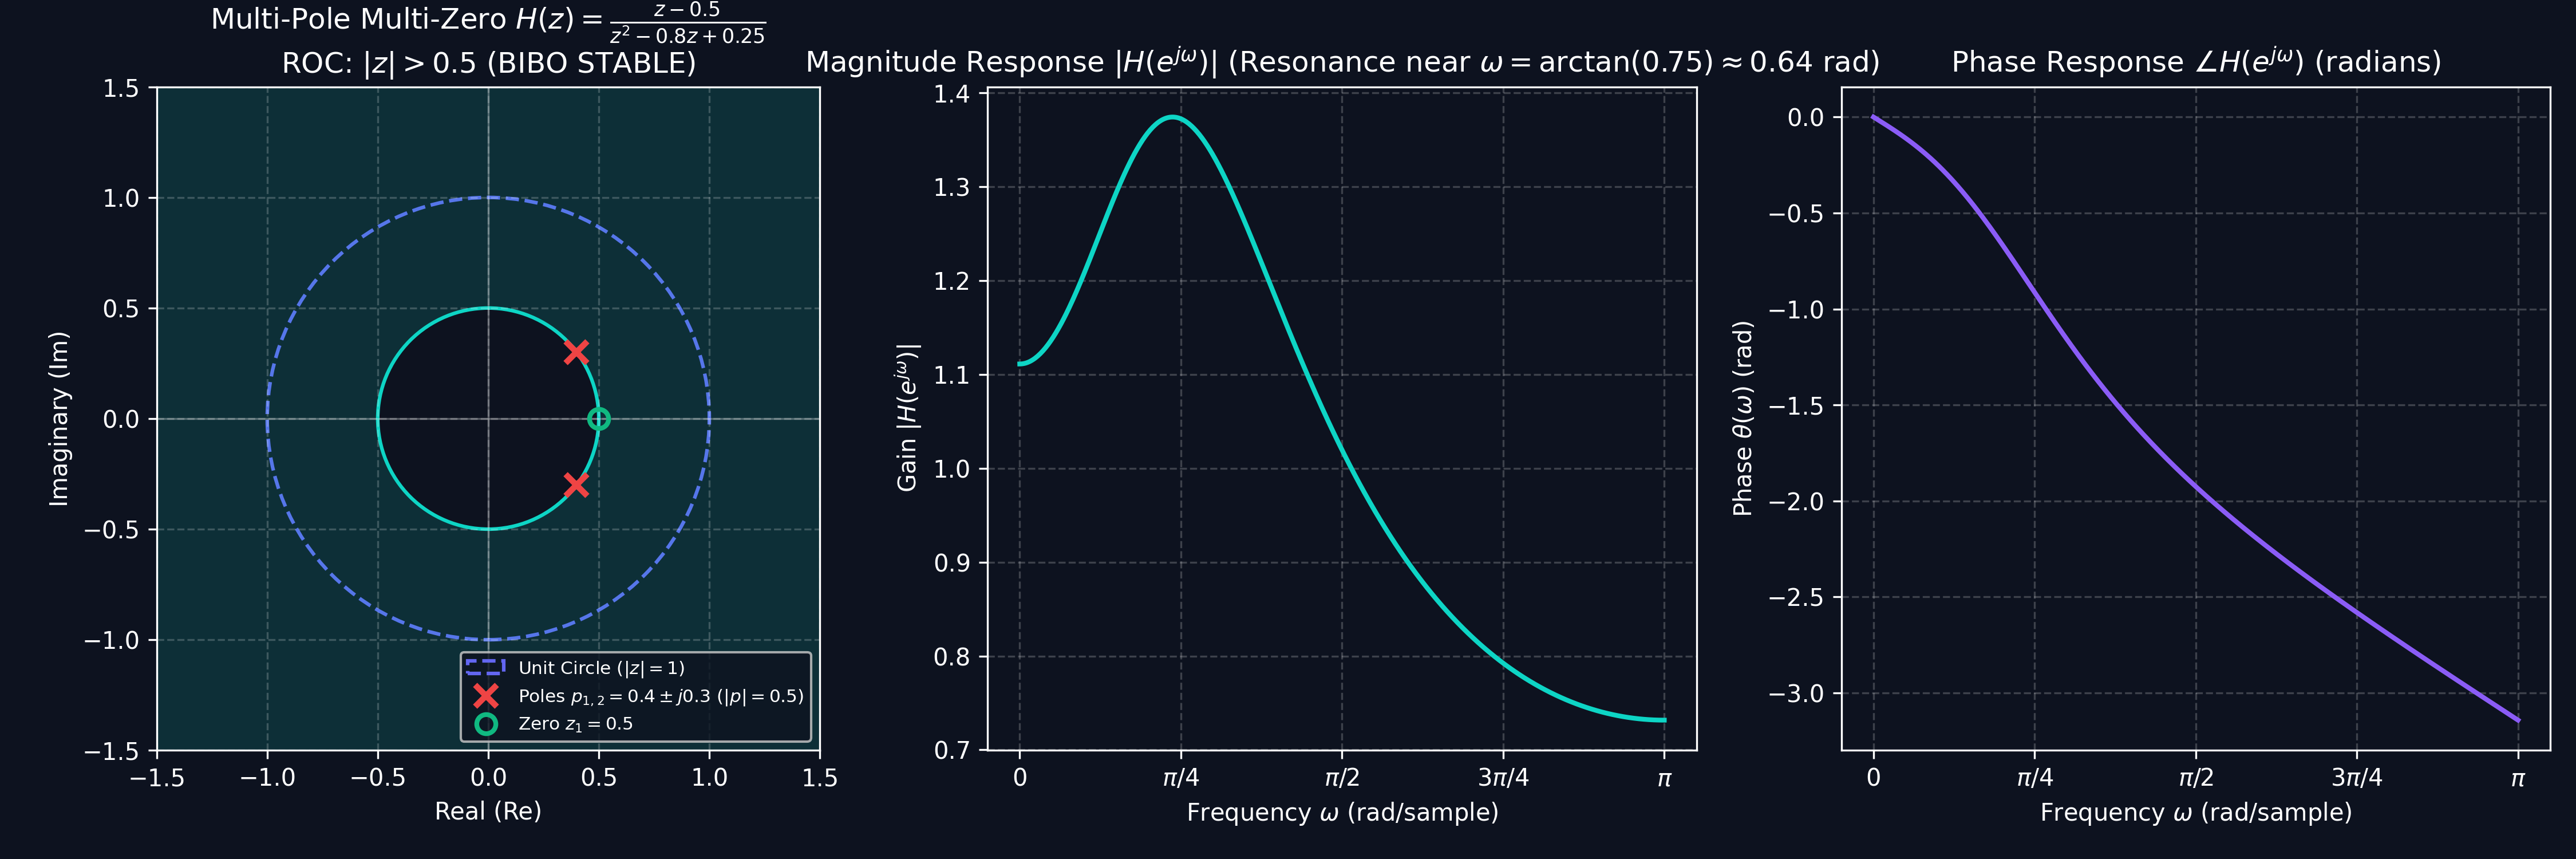
\includegraphics[width=0.95\textwidth]{images/multipole_multizero_mag_phase.png}
\caption{Multi-pole multi-zero system pole-zero plot in z-plane (left), magnitude response $|H(e^{j\omega})|$ (center), and phase response $\angle H(e^{j\omega})$ (right).}
\label{fig:multipole_system}
\end{figure}

\begin{enumerate}
    \item \textbf{Poles \& Zeros:} Zero at $z_1 = 0.5$; Complex poles at $p_{1,2} = 0.4 \pm j 0.3$ ($|p| = 0.5$).
    \item \textbf{ROC \& Stability:} Causal $\implies \mathbf{|z| > 0.5}$. Contains unit circle $|z|=1 \implies$ \textbf{BIBO STABLE}.
    \item \textbf{Magnitude Computation $|H(e^{j\omega})|$:}
    \begin{equation}
    |H(e^{j\omega})| = \frac{|e^{j\omega} - 0.5|}{|e^{j\omega} - (0.4+j0.3)| \cdot |e^{j\omega} - (0.4-j0.3)|}
    \end{equation}
    At DC ($\omega=0$): $|H(e^{j0})| = \frac{0.5}{0.45} = 1.111$ (1.09 dB). At resonance ($\omega \approx 0.6435$ rad): $|H(e^{j 0.6435})| \approx 1.54$ (3.75 dB). At $\omega=\pi$: $|H(e^{j\pi})| = \frac{1.5}{2.05} = 0.7317$ (-2.71 dB).
    \item \textbf{Phase Computation $\theta(\omega)$:}
    \begin{equation}
    \theta(\omega) = \angle(e^{j\omega} - 0.5) - \angle(e^{j\omega} - (0.4+j0.3)) - \angle(e^{j\omega} - (0.4-j0.3))
    \end{equation}
\end{enumerate}

\section{Geometric Vector Method: Magnitude \& Phase Computation}

Evaluating frequency response by moving along the unit circle $z = e^{j\omega}$:
\begin{align}
|H(e^{j\omega})| &= |C| \cdot \frac{\prod_{k=1}^M |\vec{v}_{zk}(\omega)|}{\prod_{m=1}^N |\vec{v}_{pm}(\omega)|} \\
\angle H(e^{j\omega}) &= \angle C + \sum_{k=1}^M \angle\vec{v}_{zk}(\omega) - \sum_{m=1}^N \angle\vec{v}_{pm}(\omega)
\end{align}

\subsection{\texorpdfstring{Case 1: Single Zero System ($H(z) = z - 0.6$)}{Case 1: Single Zero System}}
$|H(e^{j\omega})| = |\vec{v}_{z1}| = \sqrt{1.36 - 1.2\cos\omega}$, $\angle H(e^{j\omega}) = \text{atan2}(\sin\omega, \cos\omega - 0.6)$. Always \textbf{BIBO Stable}.

\begin{table}[H]
\centering
\small
\begin{tabular}{@{}lllll@{}}
\toprule
\textbf{Frequency $\omega$} & \textbf{Complex $z$} & \textbf{Zero Vector $\vec{v}_{z1}$} & \textbf{Magnitude $|H(e^{j\omega})|$} & \textbf{Phase $\angle H(e^{j\omega})$} \\ \midrule
$\omega = 0$ & $1 + j0$ & $0.4 + j0$ & \textbf{$0.4000$} (Min) & \textbf{$0.00^\circ$ ($0.000$ rad)} \\
$\omega = \pi/2$ & $0 + j1$ & $-0.6 + j1.0$ & \textbf{$1.1662$} & \textbf{$120.96^\circ$ ($2.111$ rad)} \\
$\omega = \pi$ & $-1 + j0$ & $-1.6 + j0$ & \textbf{$1.6000$} (Max) & \textbf{$180.00^\circ$ ($\pi$ rad)} \\
$\omega = 3\pi/2$ & $0 - j1$ & $-0.6 - j1.0$ & \textbf{$1.1662$} & \textbf{$-120.96^\circ$ ($-2.111$ rad)} \\
$\omega = 2\pi$ & $1 + j0$ & $0.4 + j0$ & \textbf{$0.4000$} (Min) & \textbf{$0.00^\circ$ ($0.000$ rad)} \\ \bottomrule
\end{tabular}
\end{table}

\begin{figure}[H]
\centering
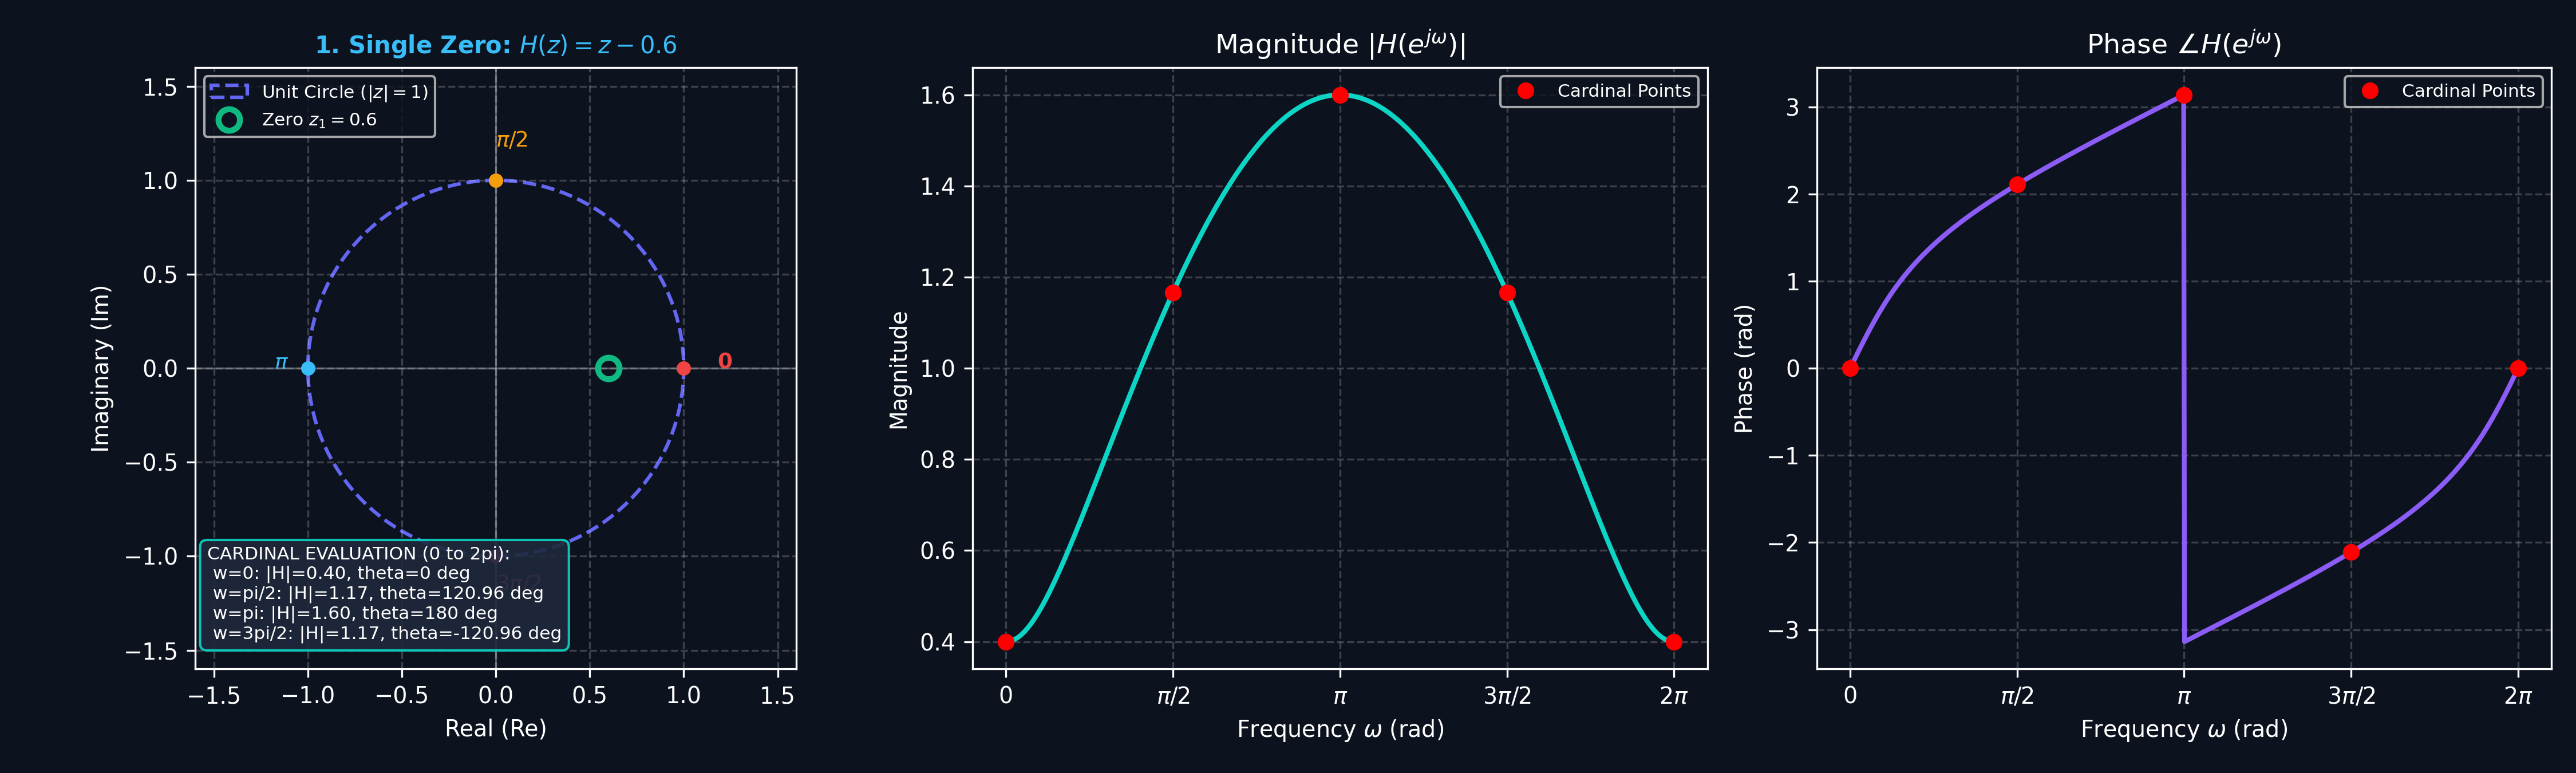
\includegraphics[width=0.95\textwidth]{images/vector_geometric_single_zero.png}
\caption{Single zero geometric vector evaluation along the unit circle from $0 \to 2\pi$.}
\label{fig:single_zero_vector}
\end{figure}

\subsection{\texorpdfstring{Case 2: Single Pole System ($H(z) = \frac{1}{z - 0.7}$)}{Case 2: Single Pole System}}
$|H(e^{j\omega})| = \frac{1}{|\vec{v}_{p1}|} = \frac{1}{\sqrt{1.49 - 1.4\cos\omega}}$. \textbf{BIBO Stable} ($|0.7|<1$).

\begin{table}[H]
\centering
\small
\begin{tabular}{@{}lllll@{}}
\toprule
\textbf{Frequency $\omega$} & \textbf{Complex $z$} & \textbf{Pole Vector $\vec{v}_{p1}$} & \textbf{Magnitude $|H(e^{j\omega})|$} & \textbf{Phase $\angle H(e^{j\omega})$} \\ \midrule
$\omega = 0$ & $1 + j0$ & $0.3 + j0$ & \textbf{$3.3333$} (Peak) & \textbf{$0.00^\circ$ ($0.000$ rad)} \\
$\omega = \pi/2$ & $0 + j1$ & $-0.7 + j1.0$ & \textbf{$0.8192$} & \textbf{$-125.00^\circ$ ($-2.182$ rad)} \\
$\omega = \pi$ & $-1 + j0$ & $-1.7 + j0$ & \textbf{$0.5882$} (Min) & \textbf{$-180.00^\circ$ ($-\pi$ rad)} \\
$\omega = 3\pi/2$ & $0 - j1$ & $-0.7 - j1.0$ & \textbf{$0.8192$} & \textbf{$+125.00^\circ$ ($+2.182$ rad)} \\
$\omega = 2\pi$ & $1 + j0$ & $0.3 + j0$ & \textbf{$3.3333$} (Peak) & \textbf{$0.00^\circ$ ($0.000$ rad)} \\ \bottomrule
\end{tabular}
\end{table}

\begin{figure}[H]
\centering
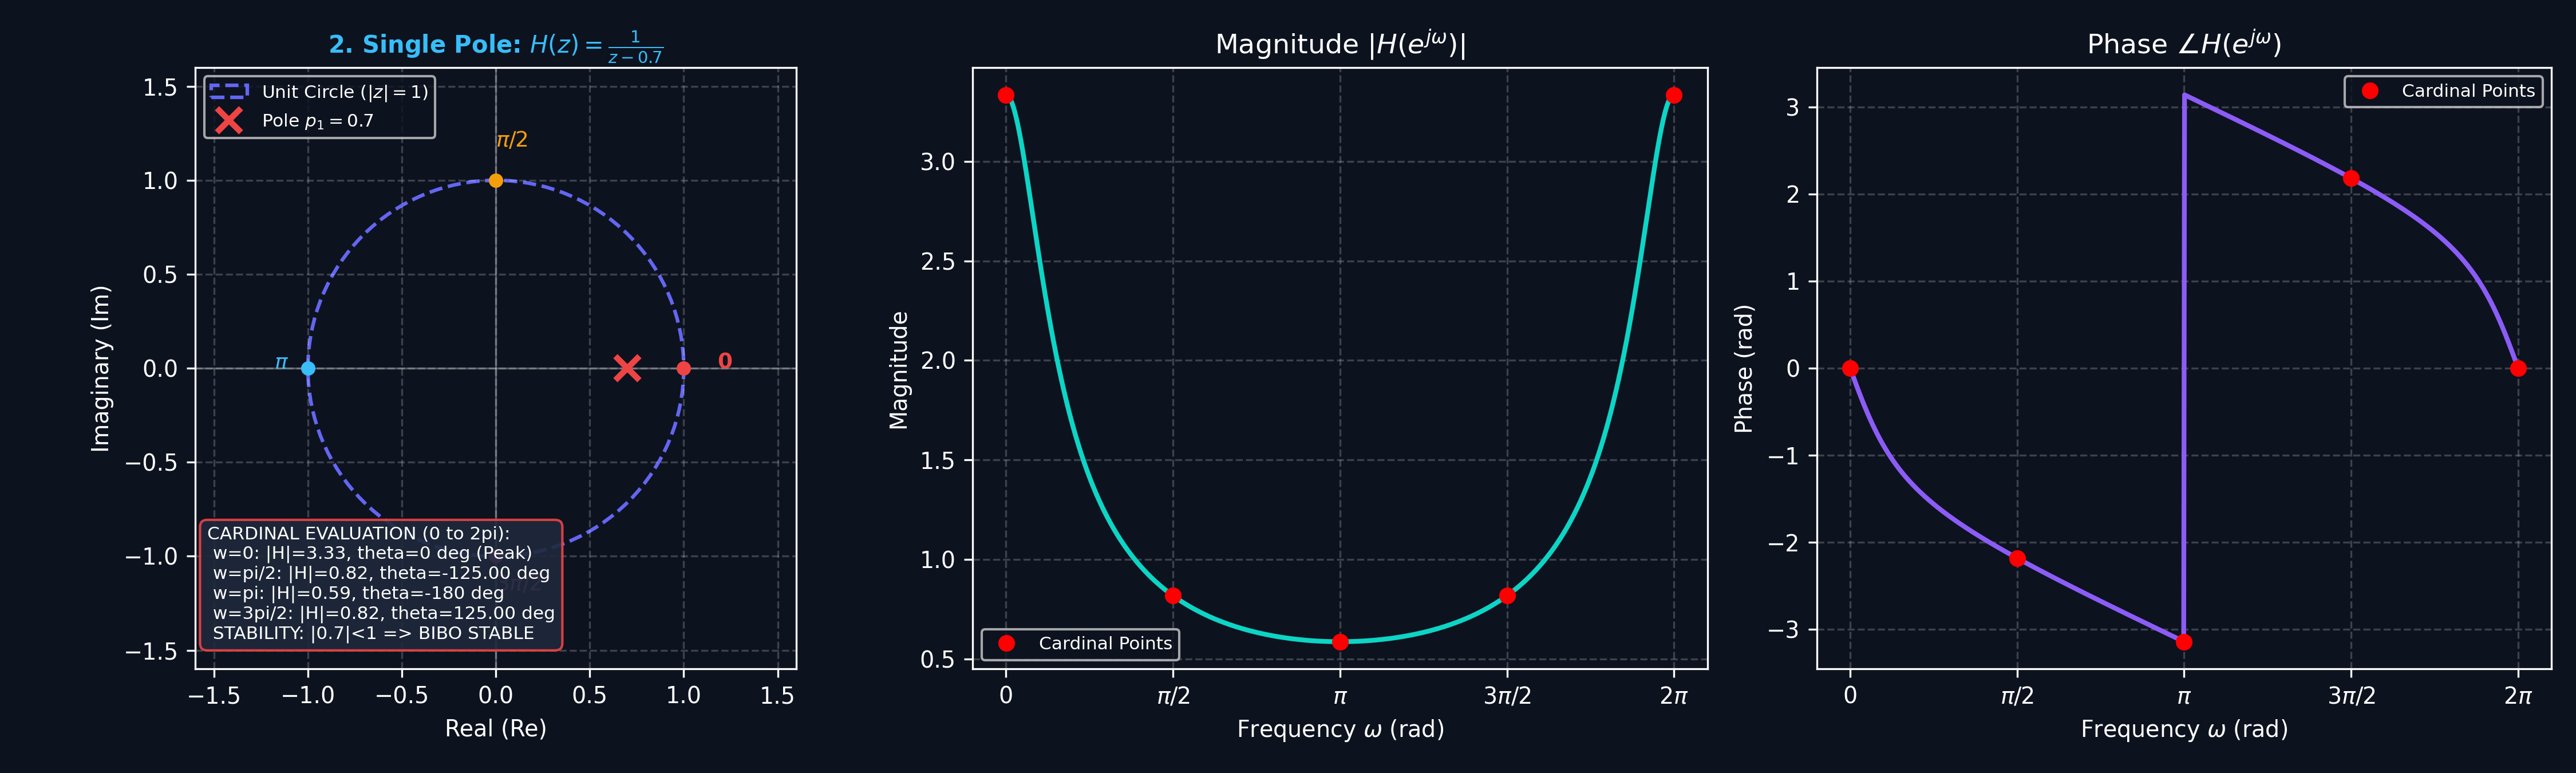
\includegraphics[width=0.95\textwidth]{images/vector_geometric_single_pole.png}
\caption{Single pole geometric vector evaluation showing resonance peak at $\omega=0$.}
\label{fig:single_pole_vector}
\end{figure}

\subsection{\texorpdfstring{Case 3: One Pole + One Zero System ($H(z) = \frac{z - 0.8}{z - 0.5}$)}{Case 3: One Pole + One Zero System}}
$|H(e^{j\omega})| = \frac{|\vec{v}_{z1}|}{|\vec{v}_{p1}|} = \sqrt{\frac{1.64 - 1.6\cos\omega}{1.25 - 1.0\cos\omega}}$, $\angle H = \theta_{z1} - \phi_{p1}$. \textbf{BIBO Stable} ($|0.5|<1$).

\begin{table}[H]
\centering
\small
\begin{tabular}{@{}lllll@{}}
\toprule
\textbf{Frequency $\omega$} & \textbf{Zero Vector $\vec{v}_{z1}$} & \textbf{Pole Vector $\vec{v}_{p1}$} & \textbf{Magnitude $|H(e^{j\omega})|$} & \textbf{Phase $\angle H(e^{j\omega})$} \\ \midrule
$\omega = 0$ & $0.2 + j0$ & $0.5 + j0$ & \textbf{$0.4000$} & \textbf{$0.00^\circ$ ($0.000$ rad)} \\
$\omega = \pi/2$ & $-0.8 + j1.0$ & $-0.5 + j1.0$ & \textbf{$1.1454$} & \textbf{$+12.09^\circ$ ($+0.211$ rad)} \\
$\omega = \pi$ & $-1.8 + j0$ & $-1.5 + j0$ & \textbf{$1.2000$} & \textbf{$0.00^\circ$ ($0.000$ rad)} \\
$\omega = 3\pi/2$ & $-0.8 - j1.0$ & $-0.5 - j1.0$ & \textbf{$1.1454$} & \textbf{$-12.09^\circ$ ($-0.211$ rad)} \\
$\omega = 2\pi$ & $0.2 + j0$ & $0.5 + j0$ & \textbf{$0.4000$} & \textbf{$0.00^\circ$ ($0.000$ rad)} \\ \bottomrule
\end{tabular}
\end{table}

\begin{figure}[H]
\centering
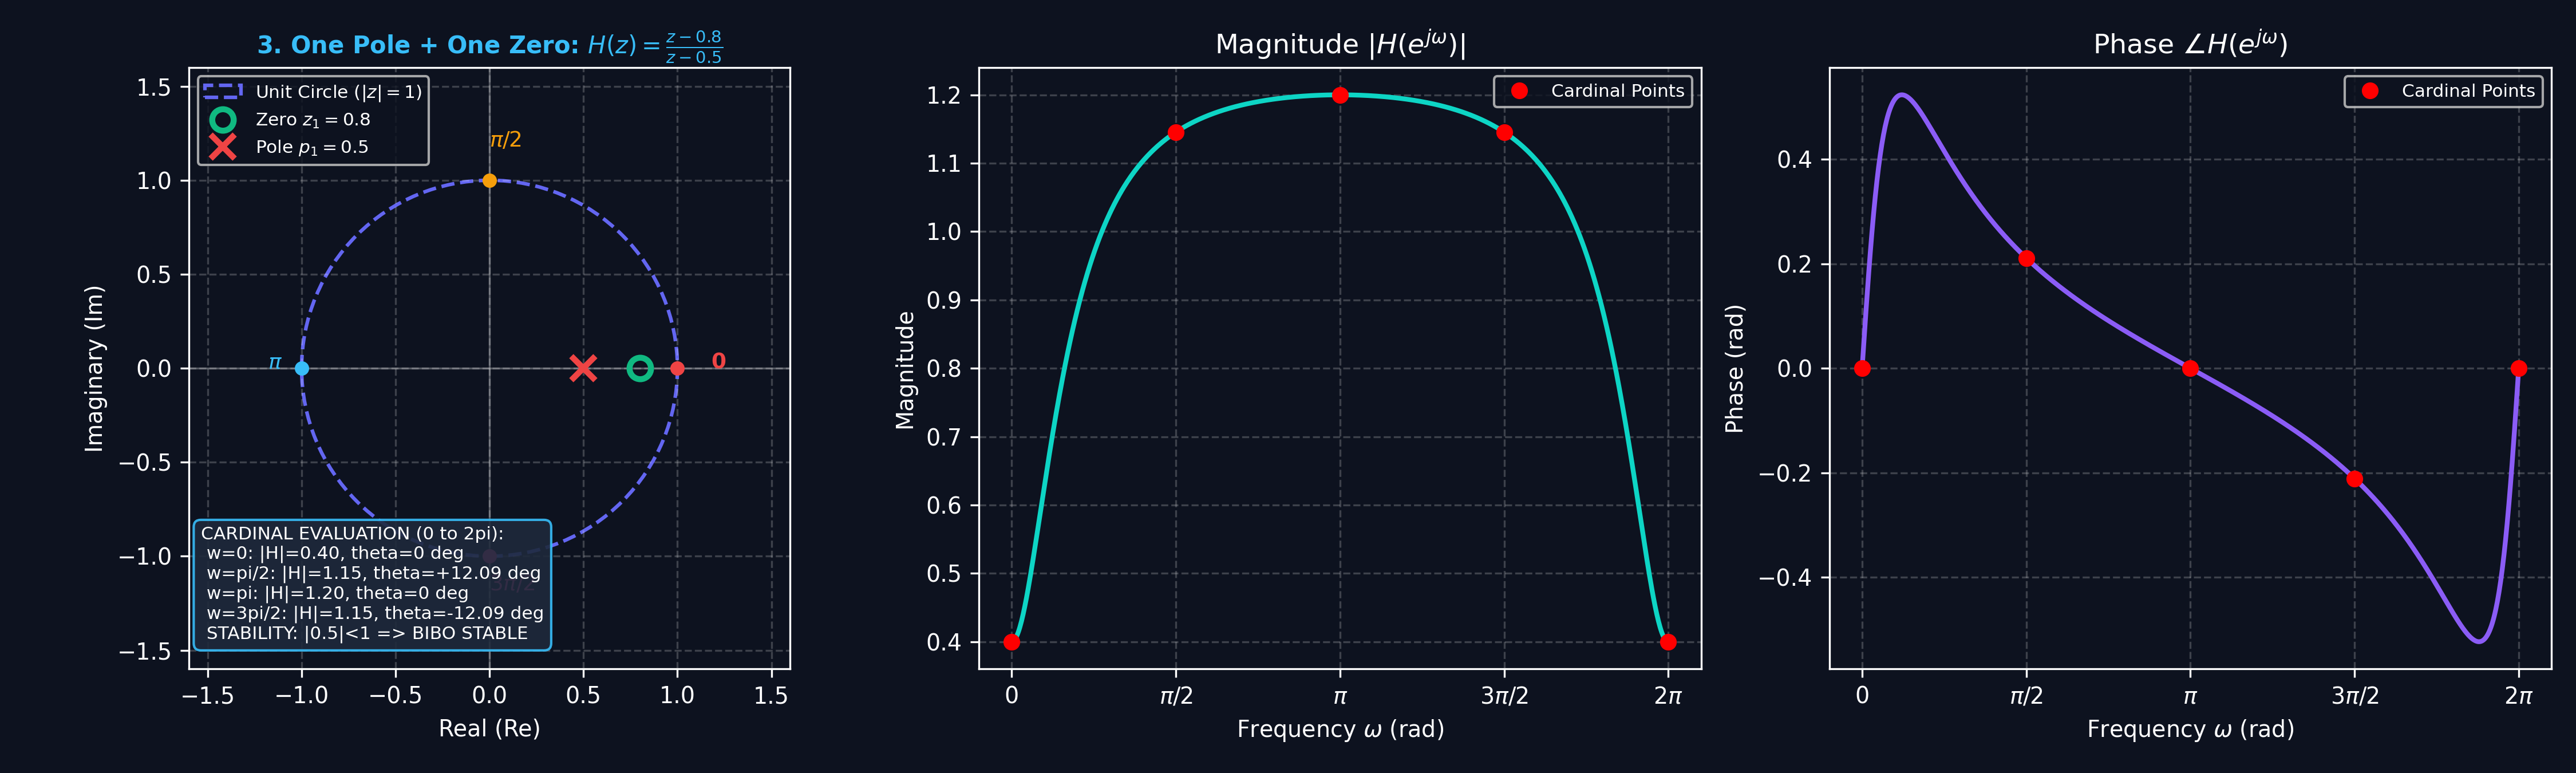
\includegraphics[width=0.95\textwidth]{images/vector_geometric_one_pole_one_zero.png}
\caption{One pole and one zero geometric vector evaluation along unit circle.}
\label{fig:one_pole_one_zero_vector}
\end{figure}

\subsection{\texorpdfstring{Case 4: Two Poles + Two Zeros System ($H(z) = \frac{z^2 - 1}{z^2 - 0.8z + 0.25}$)}{Case 4: Two Poles + Two Zeros System}}
Zeros at $z=\pm 1$ (notches at $\omega=0,\pi$), complex poles at $p_{1,2}=0.4\pm j0.3$ ($|p|=0.5$, peak at $\omega\approx 0.6435$ rad). \textbf{BIBO Stable}.

\begin{table}[H]
\centering
\small
\begin{tabular}{@{}lllll@{}}
\toprule
\textbf{Frequency $\omega$} & \textbf{Numerator $(e^{j2\omega}-1)$} & \textbf{Denominator} & \textbf{Magnitude $|H|$} & \textbf{Phase $\angle H(e^{j\omega})$} \\ \midrule
$\omega = 0$ & $0$ & $0.45$ & \textbf{$0.0000$} (Notch) & \textbf{$0.00^\circ$} \\
$\omega = \pi/2$ & $-2$ & $-0.75 - j0.8$ & \textbf{$1.8239$} & \textbf{$+133.15^\circ$ ($+2.324$ rad)} \\
$\omega = \pi$ & $0$ & $2.05$ & \textbf{$0.0000$} (Notch) & \textbf{$0.00^\circ$} \\
$\omega = 3\pi/2$ & $-2$ & $-0.75 + j0.8$ & \textbf{$1.8239$} & \textbf{$-133.15^\circ$ ($-2.324$ rad)} \\
$\omega = 2\pi$ & $0$ & $0.45$ & \textbf{$0.0000$} (Notch) & \textbf{$0.00^\circ$} \\ \bottomrule
\end{tabular}
\end{table}

\begin{figure}[H]
\centering
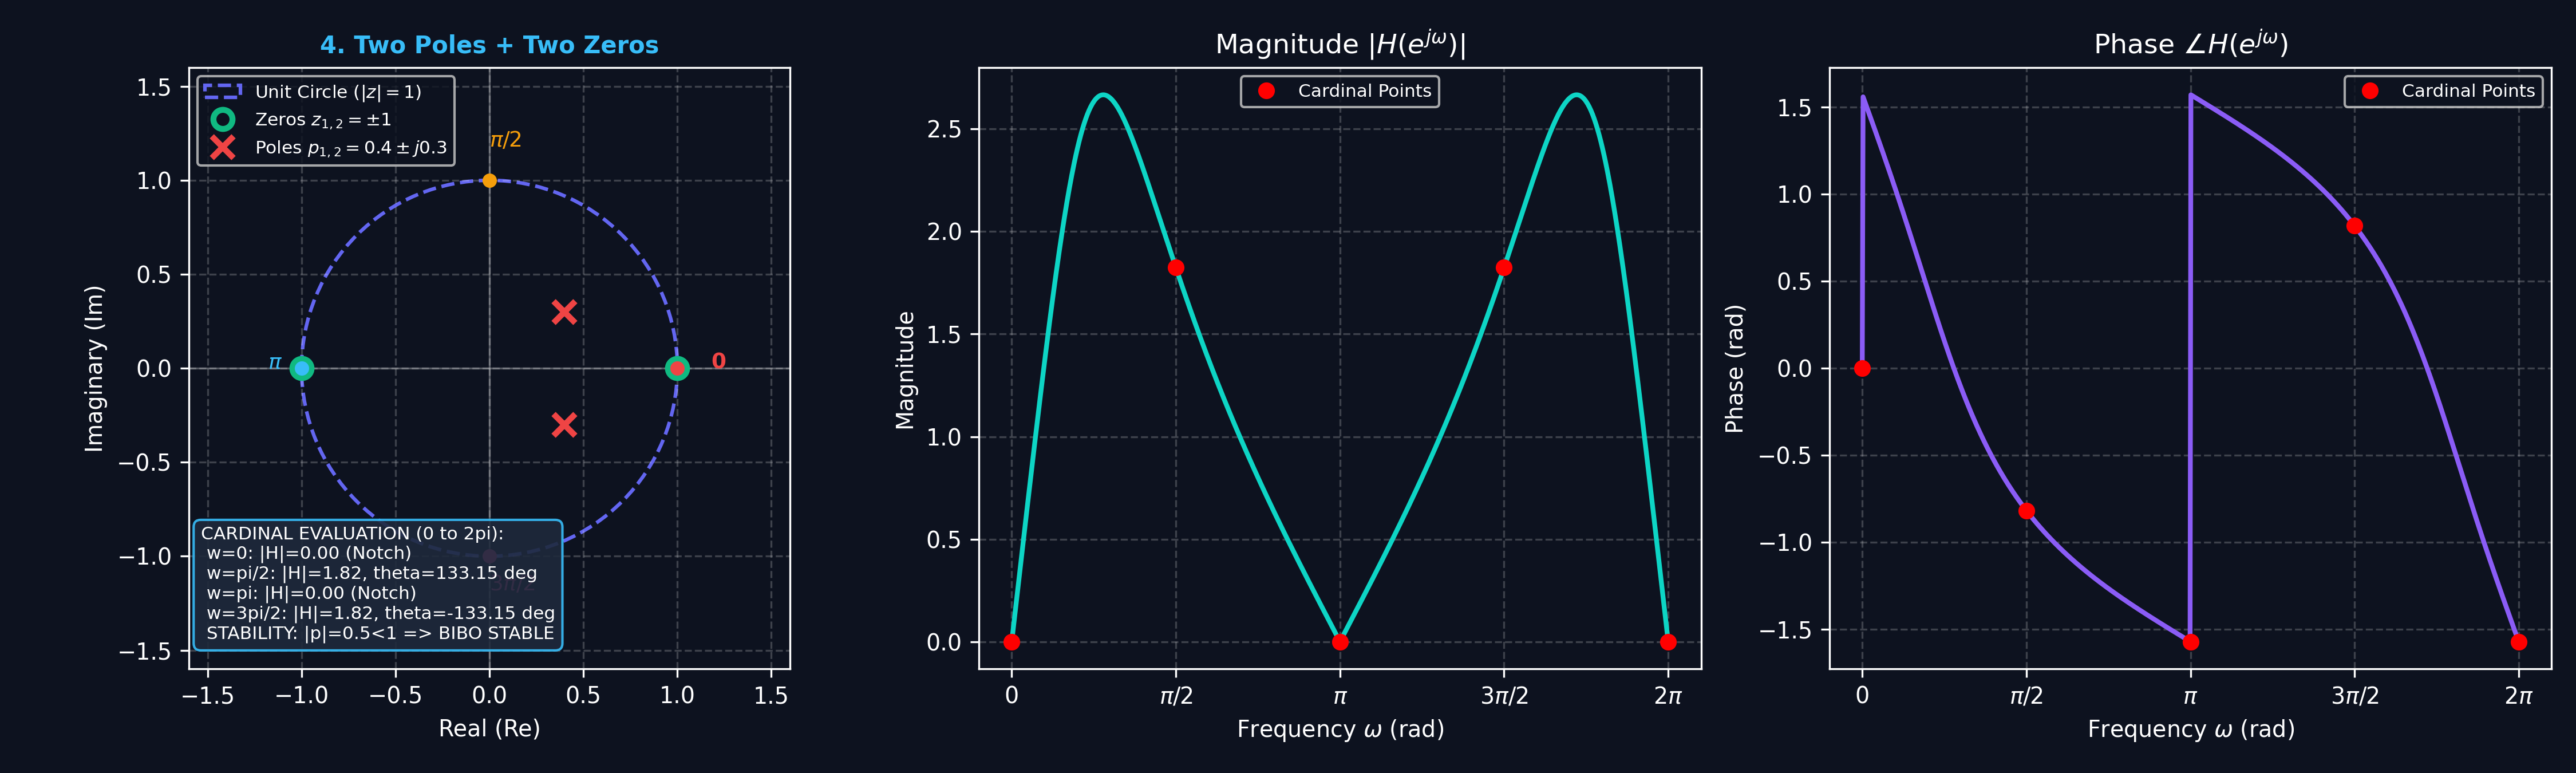
\includegraphics[width=0.95\textwidth]{images/vector_geometric_two_poles_two_zeros.png}
\caption{Two poles and two zeros geometric vector evaluation with notches and resonance.}
\label{fig:two_poles_two_zeros_vector}
\end{figure}



\section{Z-Transform Properties \& Proofs}

For $x[n] \leftrightarrow X(z)$ (ROC $R_x$) and $y[n] \leftrightarrow Y(z)$ (ROC $R_y$):

\subsection{Time Shifting}
\begin{equation}
x[n - n_0] \longleftrightarrow z^{-n_0} X(z)
\end{equation}

\subsection{Scaling in the Z-domain}
\begin{equation}
a^n x[n] \longleftrightarrow X(a^{-1} z)
\end{equation}

\subsection{Differentiation in the Z-domain}
\begin{equation}
n x[n] \longleftrightarrow -z \frac{dX(z)}{dz}
\end{equation}

\section{Comprehensive Common Z-Transform Pairs Table}

\begin{table}[H]
\centering
\small
\caption{Comprehensive Z-transform pairs with ROC and Stability comments.}
\label{tab:z_pairs}
\begin{tabular}{lllll}
\toprule
\textbf{Signal $x[n]$} & \textbf{Z-Transform $X(z)$} & \textbf{ROC} & \textbf{Poles / Zeros} & \textbf{Stability} \\
\midrule
$\delta[n]$ & $1$ & All $z$ & None & \textbf{Stable} \\
$u[n]$ & $\frac{z}{z-1}$ & $|z| > 1$ & Pole: $z=1$, Zero: $z=0$ & \textbf{Marginally Stable} \\
$a^n u[n]$ & $\frac{z}{z-a}$ & $|z| > |a|$ & Pole: $z=a$, Zero: $z=0$ & \textbf{Stable} ($|a|<1$) \\
$-a^n u[-n-1]$ & $\frac{z}{z-a}$ & $|z| < |a|$ & Pole: $z=a$, Zero: $z=0$ & \textbf{Stable} ($|a|>1$) \\
$n u[n]$ & $\frac{z}{(z-1)^2}$ & $|z| > 1$ & Double Pole: $z=1$ & \textbf{Unstable} \\
$n a^n u[n]$ & $\frac{a z}{(z-a)^2}$ & $|z| > |a|$ & Double Pole: $z=a$ & \textbf{Stable} ($|a|<1$) \\
$\cos(\omega_0 n) u[n]$ & $\frac{z(z - \cos\omega_0)}{z^2 - 2\cos\omega_0 z + 1}$ & $|z| > 1$ & Poles: $z=e^{\pm j\omega_0}$ & \textbf{Marginally Stable} \\
$\sin(\omega_0 n) u[n]$ & $\frac{z \sin\omega_0}{z^2 - 2\cos\omega_0 z + 1}$ & $|z| > 1$ & Poles: $z=e^{\pm j\omega_0}$ & \textbf{Marginally Stable} \\
$r^n \cos(\omega_0 n) u[n]$ & $\frac{z(z - r\cos\omega_0)}{z^2 - 2r\cos\omega_0 z + r^2}$ & $|z| > r$ & Poles: $z=r e^{\pm j\omega_0}$ & \textbf{Stable} ($r<1$) \\
$r^n \sin(\omega_0 n) u[n]$ & $\frac{z r \sin\omega_0}{z^2 - 2r\cos\omega_0 z + r^2}$ & $|z| > r$ & Poles: $z=r e^{\pm j\omega_0}$ & \textbf{Stable} ($r<1$) \\
\bottomrule
\end{tabular}
\end{table}

\begin{figure}[H]
\centering
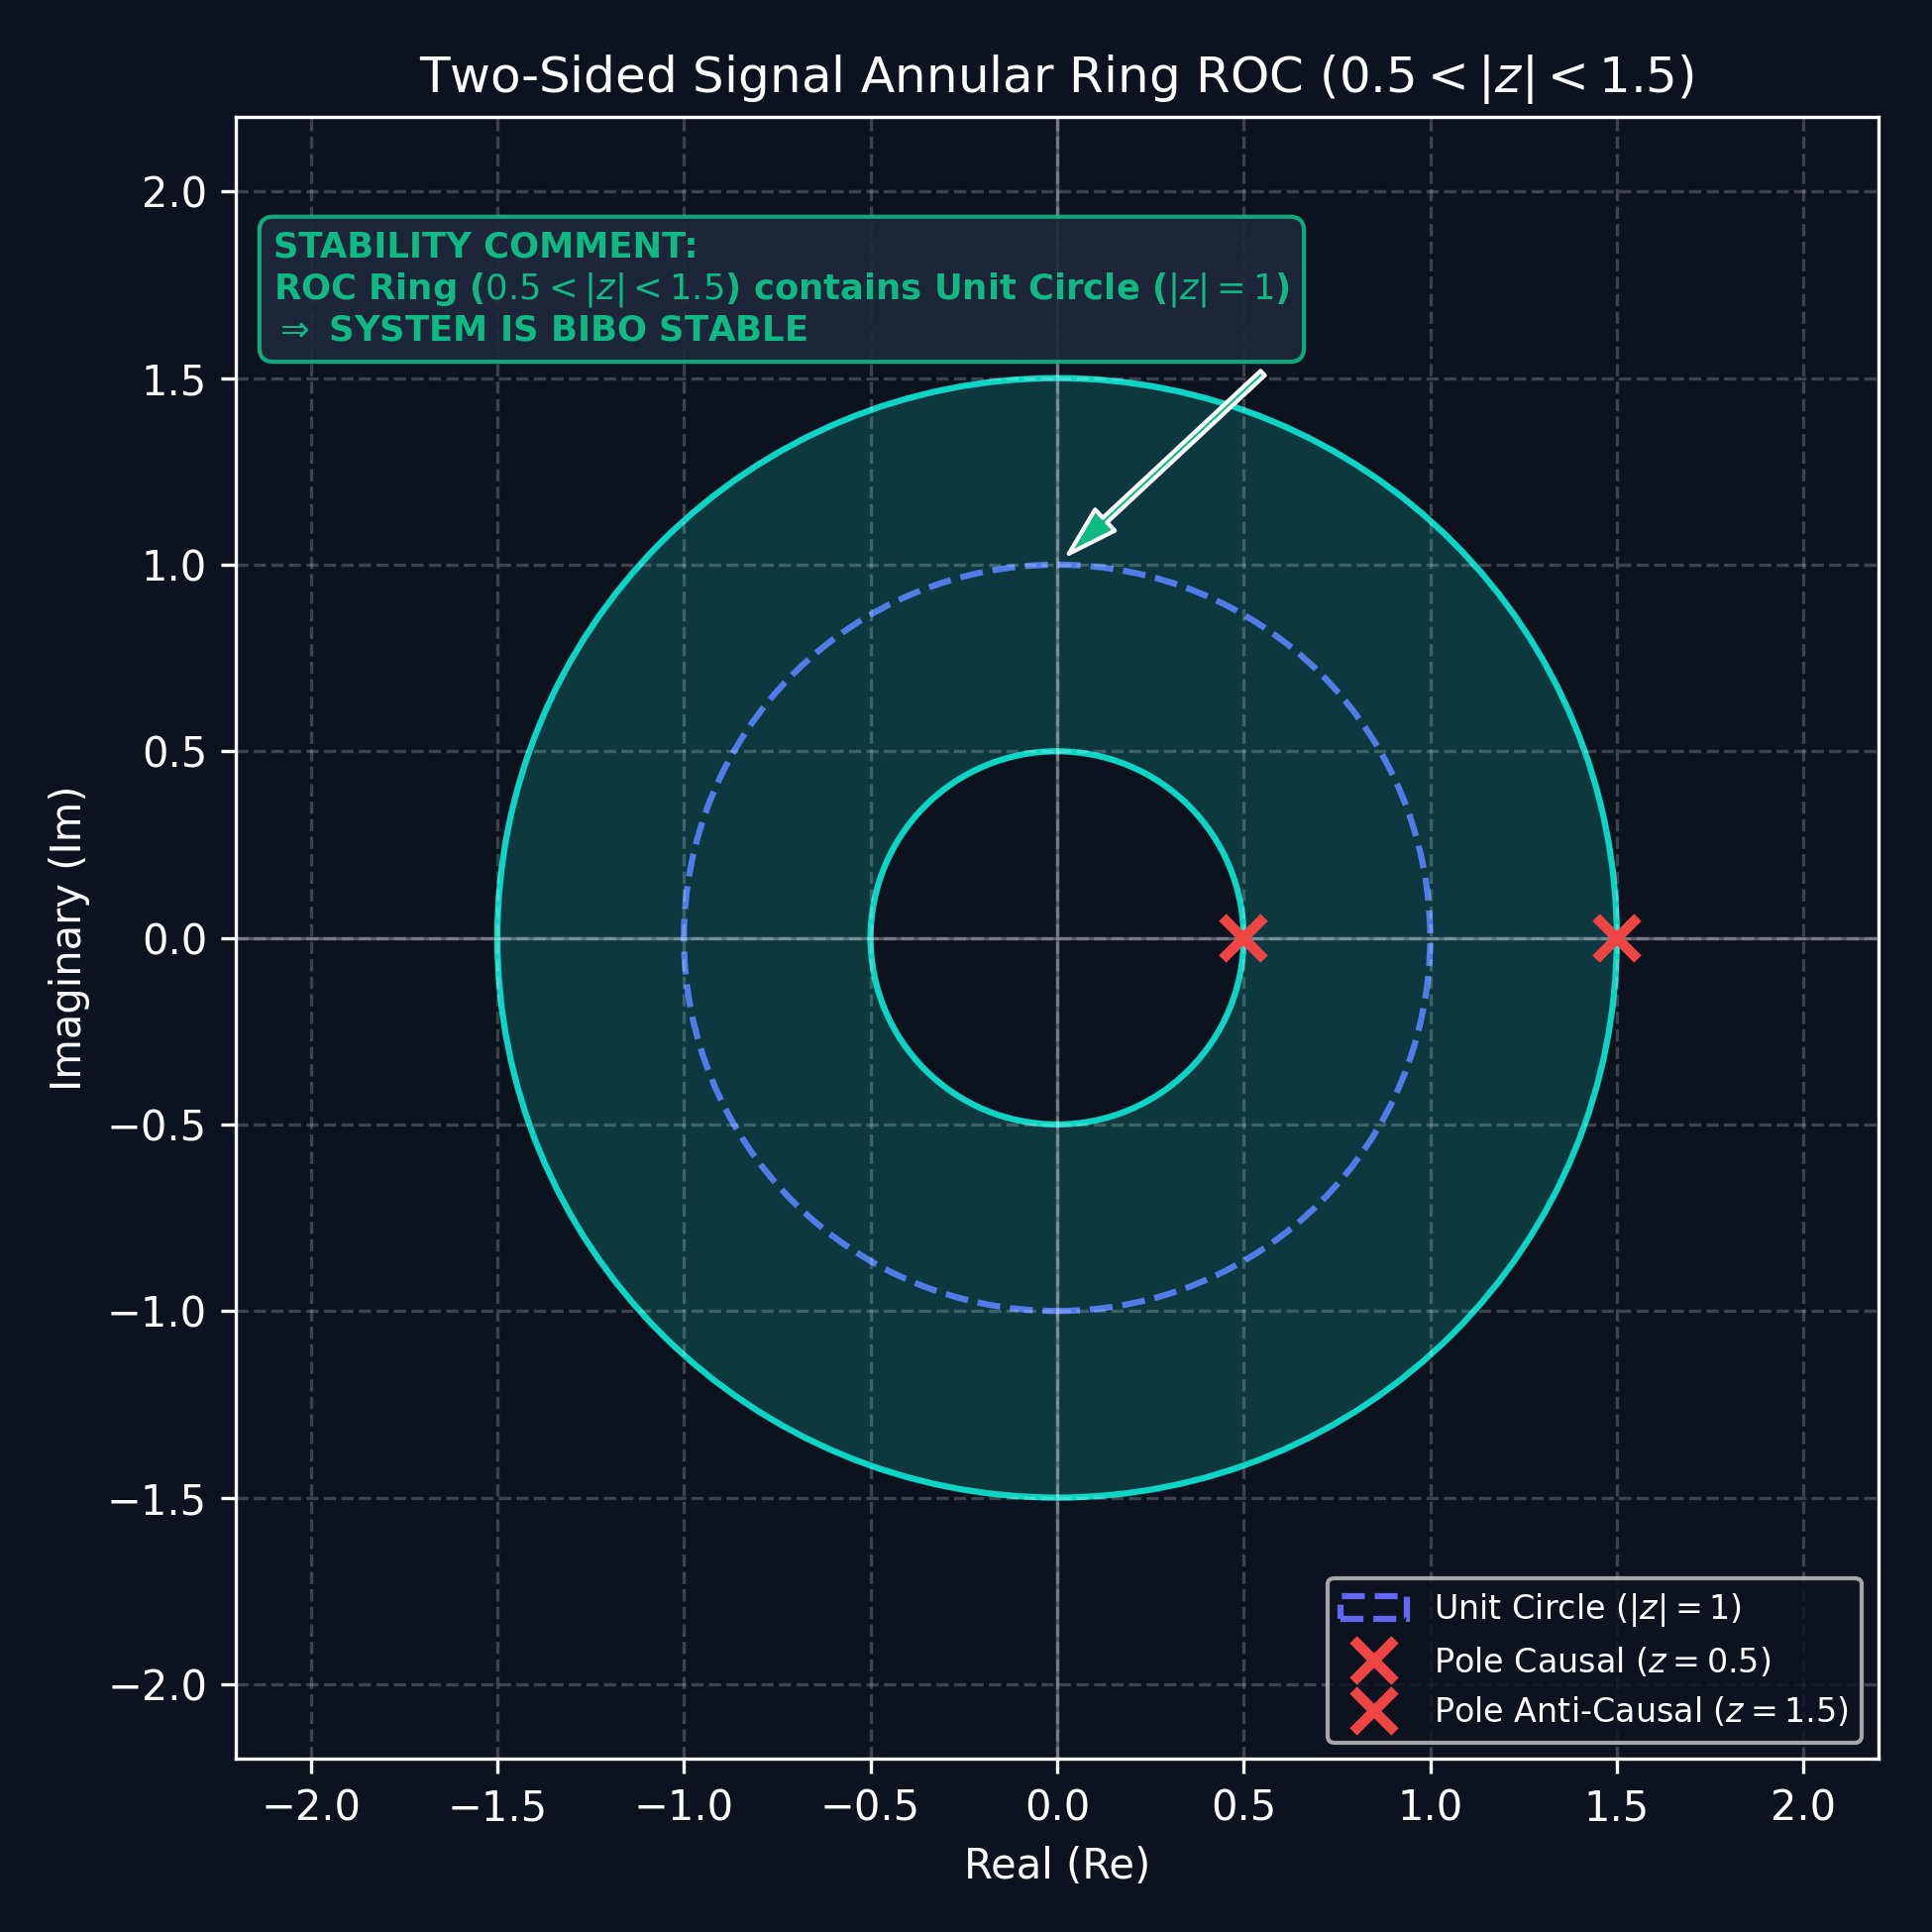
\includegraphics[width=0.45\textwidth]{images/zplane_common_pairs.png}
\caption{ROC of a stable two-sided sequence, forming an annular ring bounded by pole radii.}
\label{fig:annular}
\end{figure}

\end{document}
